% Chapter 3

\chapter{Onderzoeksmethodes} % Chapter title

\label{OnderzoeksMethode} % For referencing the chapter elsewhere, use \autoref{ch:InOnderzoek}
Zoals in de inleiding vermeld zijn er twee onderzoek benodigd om deze opdracht tot een goed einde te brengen. Voor ieder onderzoek wordt in dit hoofdstuk uitwijd over de methoden die zijn toegepast om antwoorden te verkrijgen op de vragen.
\section{Onderzoeksmethode Architectuur binnen eagleScience}
\subsection{Doel van het onderzoek}

Het doel van het onderzoek is het in kaart brengen van de dev-stack die bij Eaglescience gebruikt wordt. Deze kennis is noodzakelijk om een goede architectuur te kunnen opzetten die past binnen de huidige manier van werken maar toch de faciliteiten biedt die nodig zijn om de nieuwe oplossing bruikbaar te maken voor alle stakeholders. Daarnaast is de kennis essentieel om een module te kunnen bouwen binnen de huidige portal.


Daarnaast is door het in kaart brengen van de huidige dev-stack ook de mogelijkheid om te onderzoeken of er toevoegingen zijn die het implementeren van deze oplossing kunnen vergemakkelijken.

Om dit doel te bereiken is er als eerst een interview geweest met een senior ontwikkelaar op basis van dit interview is verder onderzocht welke bibliotheken en tools er beschikbaar zouden zijn om de nieuwe oplossing te ontwikkelen.

Het eindresultaat van dit onderzoek moet zijn dat er een duidelijk beeld is van de huidige architectuur dat binnen Eaglescience gebruikt wordt en welke mogelijkheden er zijn om de nieuwe module te integreren in de huidige portal.  Om dit resultaat te bereiken is er een onderzoeks model gemaakt en een stappenplan opgezet dat moet helpen.

\subsection{Onderzoeksmodel}
Het onderstaande onderzoeksmodel is samengesteld uit de vragen aan de linkerkant en de weg naar het resultaat van links naar rechts.\\
\begin{figure}[h!]
\myfloatalign
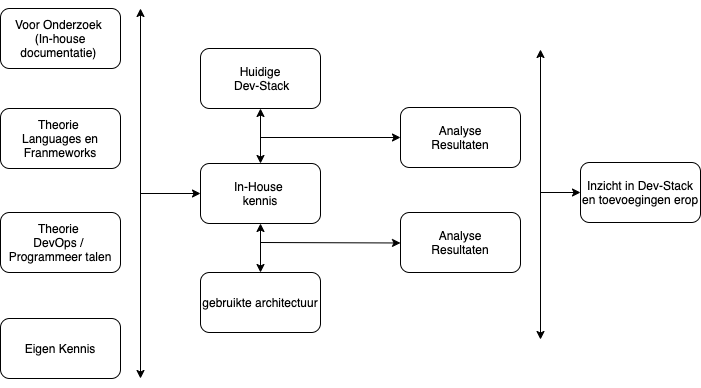
\includegraphics[width=10cm]{gfx/OnderzoeksmodelES}
\caption{Onderzoeksmodel Eaglescience}
\label{fig:Onderzoeks model Dev-Stack}
\end{figure}

\subsection{Onderzoeks vragen}
De hoofdvraag in dit onderzoek luid: \\
"Waaruit bestaat de huidige Dev-stack en welke tooling missen we om een geautomatiseerde SOUP analyse te doen?"\\
Uit deze hoofdvraag komen een aantal deelvragen:

\begin{itemize}
  \item Hoe wordt op dit moment gewerkt binnen Eaglescience en dan met name op het gebied van SOUP analyses?
  \item Welke Ontwikkeltalen gebruiken we binnen Eaglescience?
  \item Welke frameworks worden er gebruikt binnen de ontwikkeltalen?
  \item Hoe wordt op dit moment de ontwikkelde software gedeployed?
  \item Welke architectuur wordt er op dit moment gebruikt in de portal?
  \item Waar wordt de softwar uiteindelijk gedeployed?
  \item Nog veel meer vast??
\end{itemize}

\subsection{Resultaat}
Het resultaat van dit onderzoek is het hebben van een beeld hoe software op dit moment wordt ontwikkeld binnen Eaglescience en hoe deze vervolgens wordt gedeployed en waar. Ook wordt er inzicht verschaft in de mogelijkheden om de nieuwe oplossing te implementeren gezien deze een onderdeel moet gaan worden van de bestaande deploy-pipeline.
\subsection{Strategie}
De beste manier om de antwoorden op deze vragen te krijgen is door het interviewen van de ontwikkelaars en de CTO. Deze hebben op dit moment de meeste kennis van de gebruikte systemen binnen Eaglescience. Ook de verschillende "artifact files" (Package.json / build.sbt) zijn goede bronnen om te onderzoeken welke frameworks er gebruikt worden. het gaat dan voornamelijk over de build tools waar informatie uit te halen is over bibliotheken en versies hiervan.

\section{Onderzoek naar SOUP analyse}
\subsection{Doel van het onderzoek}
Het doel van dit onderzoek is het opbouwen van een theoretische basis voor het ontwikkelen van de SOUP module. Alsmede methodes om dit geautomatiseerd te kunnen doen in combinatie met databases waar kwetsbaarheden in opgeslagen zijn.


\subsection{Onderzoeksmodel}
Het onderstaande onderzoeksmodel is samengesteld uit de vragen aan de linkerkant en de weg naar het resultaat van links naar rechts.\\
\begin{figure}[h!]
\myfloatalign
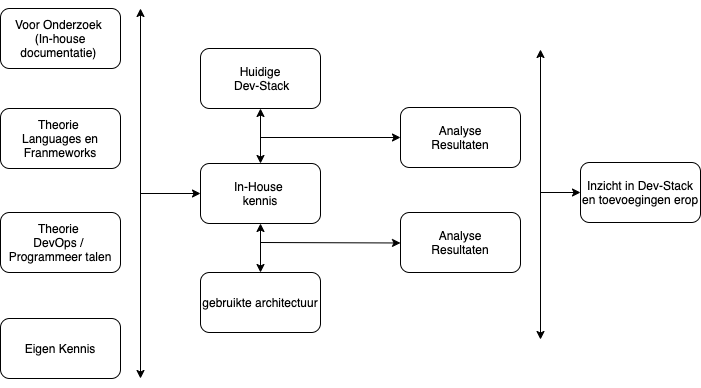
\includegraphics[width=10cm]{gfx/OnderzoeksmodelES}
\caption{Onderzoeksmodel Eaglescience}
\label{fig:Onderzoeks model Dev-Stack}
\end{figure}

\subsection{Onderzoeks vragen}
De hoofdvraag in dit onderzoek luid: \\
"Waaruit bestaat de huidige Dev-stack en welke tooling missen we om een geautomatiseerde SOUP analyse te doen?"\\
Uit deze hoofdvraag komen een aantal deelvragen:

\begin{itemize}
  \item Hoe wordt op dit moment gewerkt binnen Eaglescience en dan met name op het gebied van SOUP analyses?
  \item Welke Ontwikkeltalen gebruiken we binnen Eaglescience?
  \item Welke frameworks worden er gebruikt binnen de ontwikkeltalen?
  \item Hoe wordt op dit moment de ontwikkelde software gedeployed?
  \item Welke architectuur wordt er op dit moment gebruikt in de portal?
  \item Waar wordt de softwar uiteindelijk gedeployed?
  \item Nog veel meer vast??
\end{itemize}

\subsection{Resultaat}% is dit niet het zelfde als het doel.
Het resultaat van dit onderzoek moet zijn dat er een theoretische basis is voor het verdere verloop van het project.
\subsection{Strategie}
Dit onderzoek is voor een groot deel een bureauonderzoek uit bronnen online en boeken. Waarbij er een verslag wordt gelegd die geverifieerd wordt door de opdrachtgever..
De beste manier om de antwoorden op deze vragen te krijgen is door het interviewen van de ontwikkelaars en de CTO. Deze hebben op dit moment de meeste kennis van de gebruikte systemen binnen Eaglescience. Ook de verschillende "artifact files" (Package.json / build.sbt) zijn goede bronnen om te onderzoeken welke frameworks er gebruikt worden. het gaat dan voornamelijk over de build tools waar informatie uit te halen is over bibliotheken en versies hiervan.

\section{Tijdsverloop Onderzoeken}
Beide onderzoeken zullen parallel uitgevoerd worden zodat beide onderzoeken elkaar inzichten kunnen verschaffen. en er op die manier een beter begrip van de mogelijkheden is.
